\documentclass{article}
\usepackage[utf8]{inputenc}
\usepackage{graphicx}
%Polski
\usepackage{polski}
\usepackage[utf8]{inputenc} 
%Kod
\usepackage{listings}
\usepackage{xcolor}
\usepackage{color}
\definecolor{codegreen}{rgb}{0,0,0}
\definecolor{codegray}{rgb}{0,0,0}
\definecolor{codepurple}{rgb}{100,0,0}
\definecolor{backcolour}{rgb}{255,255,255}

\lstdefinestyle{mystyle}{
    backgroundcolor=\color{backcolour},   
    commentstyle=\color{codegreen},
    keywordstyle=\color{magenta},
    numberstyle=\tiny\color{codegray},
    stringstyle=\color{codepurple},
    basicstyle=\ttfamily\footnotesize,
    breakatwhitespace=false,         
    breaklines=false,                 
    captionpos=b,                    
    keepspaces=true,                 
    numbers=none,                    
    numbersep=5pt,                  
    showspaces=false,                
    showstringspaces=false,
    showtabs=false,                  
    tabsize=2
}

\lstset {style=mystyle}

\title{Specyfikacja Funkcjonalna}
\author{Ochnio Szymon i Sekula Sebastian}
\date{March 2022}


\begin{document}
\maketitle

\section{Opis Ogólny}
\subsection{Nazwa Programu}
GGAPF (Graph Generator and Path Finder)
\subsection{Poruszany problem}
Program będzie w stanie generować graf składający się z węzłów według określonej wielkości kolumn oraz wierszy, a także przypisywać do krawędzi wagi z~określonego przedziału. Umożliwi również podział grafu na spójne podgrafy. Na główne zadania programu będzie składało się sprawdzenie spójności grafu przy pomocy algorytu BFS oraz znalezenienie najkrótszej ścieżki między dwoma zadanymi wierzchołkami za pomocą algorytmu Dijkstry.

\section{Opis Funkcjonalności}
\subsection{Jak korzystać z programu?}
Program jest przystosowany do uruchamiania na systemach opartych o architekturę Linux.
Program należy skompilować korzystając z komendy "make" (Można ją zainstalować wpisując: "sudo apt install make" w terminalu) w folderze z~projektem, .
Następnie program należy uruchomić z linii poleceń wpisując "./ggapf.out \textless lista\mathunderscore parametrów\textgreater". Możliwe paramtery opisane są w dalszej części specyfikacji.
\subsection{Uruchomienie programu}
Wywołanie: 
\begin{lstlisting}
./ggapf.out [-h --help | -help | -?] [-s source_file]
[-x x_columns] [-y y_rows] [-n n_subgraphs] [-b begin_node] 
[-e end_node] [-r result_file] [-f from_weight] [-t to_weight]
\end{lstlisting}

\newpage
Flagi:
\begin{itemize}
    \item brak argumentów lub argumenty inne niż opisane poniżej - program wyświetla informację o niepoprawnej ilości argumentów i uruchamia podręcznego helpa.
    \item -h \textbar--help  \textbar-help \textbar-? - wyświetla podręcznego helpa
    \item -s source\_file - nazwa pliku źródłowego (użycie tej flagi sprawia, że podanie wartości dla flag -x i -y nie będzie miało znaczenia, bo ilość wierszy oraz kolumn zostanie wczytana z pierwszej linii podanego pliku)
    \item -x x\_columns - liczba kolumn węzłów w grafie. Wartość domyślna: 5.
    \item -y y\_rows - liczba wierszy węzłów w grafie. Wartość domyślna: 5.
    \item -n n\_subgraphs - pozwala podzielić graf na spójne i rozłączne względem siebie grafy. ${1 \leq n \leq (x*y)/2}$ (wielkość zmiennej domyślniej jest ustawiona na 1, graf nie jest dzielony na żadne podgrafy, wpisanie wartości mniejszej od 1 traktowane jest jako błąd). Flaga nie ma zastosowania w momencie, kiedy wczytany przez użytkownika graf jest niespójny, program da o tym znać stosownym komunikatem.
    \item -b begin\_node - węzeł początkowy szukanej ścieżki. \newline [FLAGA OBOWIĄZKOWA]
    \item -e end\_node - węzeł końcowy szukanej ścieżki. \newline [FLAGA OBOWIĄZKOWA]
    \item -r result\_file - nazwa pliku docelowego
    \item -f from\_weight - początek zakresu wag (włącznie). Wartość domyślna: 1.0 (kropka jako separator dziesiętny)
    \item -t to\_weight - koniec zakresu wag (włącznie). Wartość domyślna: 10.0. (kropka jako separator dziesiętny)
    
\end{itemize}
\subsection{Możliwości programu}
\begin{itemize}
    \item Generuje graf o podanych parametrach (zadana wielkość, zakres wag dla krawędzi)
    \item Wczytuje graf z podanego przez użytkownika pliku o określonym formacie
    \item Potrafi zbadać czy graf jest spójny (korzystając z algorytmu BFS).
    \item Potrafi podzielić graf na n spójnych podgrafów.
    \item Znajduje najkrótszą ścieżkę między dwoma wierzchołkami (przy pomocy algorytmu Dijkstry)
    \item Zapisuje graf do pliku o podanej przez użytkownika nazwie oraz rozszerzeniu.
\end{itemize}

\section{Format Danych i Struktura Plików}

\subsection{Słownik}

\begin{tabular}{|c|p{28em}|}
\hline
\textbf{termin} & \textbf{definicja} \\
\hline
node & węzeł w grafie \\
\hline
source\_file & plik źródłowy z którego został pozyskany graf \\
\hline
result\_file & plik wynikowy zawierające (przetworzony) przetworzony graf \\
\hline
weight & waga, znajdująca się na krawędziach pomiędzy węzłami \\
\hline
subgraphs & podgrafy powstałe w wyniku skorzystania z flagi "-n" przy uruchamianiu programu, to jest podzieleniu grafu spójnego na x elementów \\
\hline
row & wiersz \\
\hline
column & kolumna \\
\hline
make & komenda będąca składową paczki "make", wykorzystywana do szybkiej kompilacji programu. \\
\hline
stdout & standardowe wyjście, terminal.\\
\hline
\end{tabular}

\subsection{Struktura katalogów}
Folder z programem zawiera 3 katalogi:
\\
bin - przechowuje wszystkie pliki powstałe w wyniku kompilacji kodu.
\\
src - przechowuje wszystkie pliki, które zawierają jakikolwiek kod.
\\
data - przechowuje przykładowe, wcześniej spreparowane grafy.

\subsection{Dane wejściowe}
Dane wejściowe przekazywane jako parametry uruchomienia zostały opisane w~punkcie 2.2.
W tym punkcie opisany jest jedynie format pliku z danymi. Plik wejściowy może mieć dowolne rozszerzenie, ale musi być zapisany z kodowaniem ASCII. Format danych w pliku powinien wyglądać w sposób następujący:
\begin{lstlisting}
3 2
1:0.263 3:0.865
0:0.263 4:0.920 2:0.876
1:0.876 5:0.213
0:0.865 4:0.007
3:0.007 1:0.920 5:0.017
4:0.017 2:0.213
\end{lstlisting}
W pierwszym wierszu są dane kolejno: liczba wierszy, a następnie kolumn - zapis "3 2" oznacza graf o 3 kolumnach i 2 wierszach.
\\
W kolejnych wierszach pliku jest zawarta lista sąsiedztwa (zaczynająca się od zerowego węzła) zawierająca informacje o połączeniach między węzłami. Przykładowo zapis "1:0.263 3:0.865" oznacza, że z węzła 0 wychodzą krawędzie do węzła 1 o wadze 0.263 i do węzła 3 o wadze 0.865. Jako separtor dziesiętny wymagany jest znak kropki (".")

\newpage
Wizualizacja całego opisywanego grafu:
{\centering{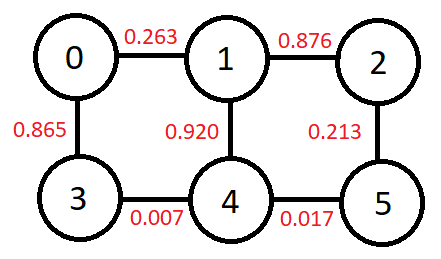
\includegraphics[scale=0.7]{graph1}} \\ }

\subsection{Dane wyjściowe}
\begin{itemize}
\item Program wypisuje na stdout informacje o ewentualnych ostrzeżeniach i błędach.
\item Program wypisuje na stdout informacje o tym czy podany graf jest spójny.
\item Program wypisuje na stdout długość najkrótszej ścieżki między zadanymi wierzchołkami.
\item Jeśli użytkownik podał parametr "-r", graf wynikowy zostanie zapisany do podanego przez użytkownika pliku w postaci listy sąsiedztwa (format danych opisany w sekcji "Dane wejściowe"). W przeciwnym wypadku graf zostanie wypisany na stdout.
\end{itemize}
\section{Scenariusz Działania Programu}

\subsection{Scenariusz ogólny}
Program po uruchomieniu sprawdza poprawność podanych argumentów. 
\\
Jeżeli zostanie podany plik źródłowy, sprawdzana jest spójność grafu wejściowego przy pomocy algorytmu BFS. Jeżeli graf jest niespójny nie istnieje możliwość podzielenia go na więcej podgrafów, w przeciwnym wypadku następuje podział na n podgrafów.
\\
Jeżeli plik wejściowy nie zostanie podany, następuje wygenerowanie grafu według zadanych parametrów.
\\
W dalszym ciągu program szuka przy pomocy algorytmu Dijkstry najkrótszej ścieżki dla zadanych dwóch wierzchołków wyświetla jej długość i przebieg lub informację o jej braku (np. gdy wskazane wierzchołki znajdują się w oddzielnych podgrafach).
\\
W dalszej kolejności ewentualnie przekształcony graf jest zapisywany do pliku lub wypisywany na standardowe wyjście.

\subsection{Scenariusz szczegółowy}
\begin{enumerate}

\item Czy została podana flaga -s ?
    \begin{itemize}
        \item Tak - Czy udało się wczytać source\_file?
        \begin{itemize}
            \item Tak - Następuje wczytanie grafu z podanego pliku do programu. Flagi -x i -y zostaną zignorowane.
            \item Nie - program wyświetla komunikat o błędzie i kończy swoje działanie.
        \end{itemize}
        \item Nie - Graf jest generowany według podanych -x, -y, -n i zakresu wag.
    \end{itemize}
    
\item Program sprawdza czy wczytany graf jest spójny przy pomocy algorytmu BFS.

\item Czy została podana flaga -n ?
    \begin{itemize}
        \item Tak - jeśli graf jest spójny następuje podział grafu na wskazaną liczbę podgrafów. W przypadku, kiedy graf nie jest spójny następuje informacja o tym, że nie można podzielić tego grafu na wskazaną liczbę podgrafów.
    \end{itemize}

\item Czy zostały wykorzystane flagi -b -e ?
    \begin{itemize}
        \item Tak - program przy użyciu algorytmu Dijkstry znajdzie najkrótszą ścieżkę między podanymi wierzchołkami, wypisze jej długość i pokaże przebieg.
        \item Nie - program wyświetla komunikat o błędzie i kończy swoje działanie.
    \end{itemize}

\item Czy została podana flaga -r ?
    \begin{itemize}
        \item Tak - graf zostaje zapisany do pliku o podanej nazwie w postaci listy sąsiedztwa.
        \item Nie - graf zostaje wypisany na standardowe wyjście.
    \end{itemize}
    
\end{enumerate}

\section{Przykłady}

Przykładowe pliki z danymi przechowywane są w folderze "data":
\begin{enumerate}
    \item graf1.txt - plik zawierający niewielki (5x5) graf niespójny z poprawnymi danymi
    \item graf2.txt - plik zawierający większy (10x10) graf spójny z poprawnymi danymi
    \item graf3.txt - plik zawierający graf z danymi w niepoprawnym formacie
\end{enumerate}
Program z przykładowymi plikami można uruchomić poleceniem "make graf1" dla pliku graf1.txt analogicznie dla pozostałych plików przykładowych.
\\\\
Wymienione niżej przypadki, można tworzyć wykorzystując już wcześniej spreparowany plik 'Makefile'.
\\\\
Mają one za zadanie pokazać:
\begin{enumerate}
    \item Wczytywanie danych
    \item Sprawdzanie przez program spójności grafu.
    \item Sprawdzanie czy istnieje ścieżka pomiędzy podanymi wierzchołkami.
    \item Liczenie najkrótszej ścieżki między podanymi wierzchołkami.
    \item Wskazywanie przebiegu najkrótszej ścieżki.
    \item Wypisywanie grafu na wyjście.
    \item Reakcję na zły format danych w pliku.
\end{enumerate}

\end{document}
